\section{Giới thiệu đề tài}

\subsection{Giới thiệu đề tài và cơ sở lý thuyết}

\subsubsection{Giới thiệu đề tài}

\hspace{0.5cm} Đồ án tốt nghiệp thuộc ngành Kỹ thuật Máy tính, thuộc chương trình Đào tạo Kỹ sư Khoa học Máy tính (CO4347), đề tài "Xây dựng thuật toán tính toán tọa độ mục tiêu từ dữ liệu GPS, góc ngắm và khoảng cách", với phần mở rộng là "Tracking mục tiêu di động thời gian thực với đa cảm biến Laser-IMU-GNSS".

Trong giai đoạn 1, nhóm đã xây dựng thành công thuật toán tính toán tọa độ mục tiêu ở trạng thái tĩnh. Hệ thống nhận đầu vào là vị trí GPS của người quan sát, góc ngắm (azimuth, elevation) đo từ cảm biến quán tính (IMU), và khoảng cách đo bằng máy đo khoảng cách laser. Đầu ra là tọa độ địa lý (kinh độ, vĩ độ, cao độ) của mục tiêu. Thuật toán được chạy theo từng điểm riêng lẻ (single-point): mỗi lần tính toán là một lần đọc cảm biến riêng biệt, không có sự liên kết giữa các lần đo về mặt thời gian. Kết quả giai đoạn 1 đã được kiểm chứng bằng 104 test tự động và đánh giá trên giao diện bản đồ số.

Giai đoạn 2 (Phase 2) mở rộng bài toán đáng kể: mục tiêu không còn đứng yên mà có thể di chuyển với tốc độ và hướng thay đổi theo thời gian. Hệ thống phải tính toán liên tục, cập nhật vị trí mục tiêu theo thời gian thực và hiển thị quá trình di chuyển trên bản đồ số. Yêu cầu này đòi hỏi xử lý dòng dữ liệu cảm biến liên tục, kết hợp nhiều nguồn cảm biến và áp dụng các bộ lọc ước lượng (estimation filter) để xác định vị trí chính xác ngay cả khi tín hiệu bị nhiễu hoặc gián đoạn.

Một thay đổi quan trọng trong giai đoạn 2 là mô hình triển khai. Trong giai đoạn 1, thuật toán chạy trực tiếp trên trình duyệt web. Giai đoạn 2 chuyển sang mô hình máy chủ kết hợp trình duyệt: phía máy chủ xử lý thuật toán và quản lý trạng thái, phía giao diện hiển thị bản đồ và điều khiển. Kiến trúc này phản ánh thiết kế thực tế của hệ thống theo dõi, nơi thiết bị nhúng (Raspberry Pi) gửi dữ liệu cảm biến lên máy chủ trung tâm, máy chủ xử lý và trả kết quả về giao diện người dùng.

So với giai đoạn 1, đồ án hiện tại khác biệt căn bản ở chỗ duy trì trạng thái bộ lọc liên tục qua nhiều chu kỳ, xử lý nhiều phiên đồng thời và hiển thị kết quả trên bản đồ theo thời gian thực, thay vì tính một điểm tọa độ duy nhất cho mỗi lần đọc cảm biến.
\subsubsection{Phát biểu bài toán}

\hspace{0.5cm} Bài toán được phát biểu như sau: Cho một người quan sát mang thiết bị GNSS (GPS), cảm biến IMU, và máy đo khoảng cách laser. Người quan sát này hướng thiết bị về phía mục tiêu đang di chuyển. Tại mỗi thời điểm $k$, hệ thống cần thực hiện các nhiệm vụ sau:

\begin{enumerate}
    \item \textbf{Xác định vị trí người quan sát}: Lấy tọa độ tuyệt đối (kinh độ $\lambda$, vĩ độ $\phi$, cao độ $h$) từ thiết bị GNSS. GPS dân sự tiêu chuẩn có độ chính xác 2 đến 5 m ở điều kiện ngoài trời tốt.
    \item \textbf{Đo góc ngắm}: Lấy góc azimuth $\alpha$ (góc giữa hướng Bắc và hướng ngắm, tính theo chiều kim đồng hồ từ 0\textdegree{} đến 360\textdegree{}) và góc elevation $\beta$ (góc cao so với mặt phẳng ngang, từ $-90$\textdegree{} đến $+90$\textdegree{}) từ cảm biến IMU. Cảm biến quán tính có tần số cao (100 đến 1000 Hz) nhưng bị trôi (drift) theo thời gian.
    \item \textbf{Đo khoảng cách}: Lấy khoảng cách thực tế từ người quan sát đến mục tiêu bằng máy đo laser rangefinder. Độ chính xác cao ($\pm 1$ đến 2 cm) nhưng bị giới hạn bởi tầm xa và yêu cầu tầm nhìn thẳng (Line-of-Sight).
    \item \textbf{Tính toán tọa độ mục tiêu}: Từ ba đại lượng trên, tính toán tọa độ 3D (kinh độ, vĩ độ, cao độ) của mục tiêu trong hệ tọa độ WGS-84 thông qua chuỗi chuyển đổi WGS-84 $\rightarrow$ ECEF $\rightarrow$ ENU.
    \item \textbf{Lọc và ước lượng}: Áp dụng bộ lọc Kalman \cite{kalman1961new} hoặc bộ lọc alpha-beta để ước lượng vị trí và vận tốc của mục tiêu, giảm ảnh hưởng của nhiễu cảm biến.
    \item \textbf{Hiển thị thời gian thực}: Truyền kết quả lên giao diện web qua kênh truyền dữ liệu hai chiều và hiển thị vị trí, quỹ đạo mục tiêu trên bản đồ số.
\end{enumerate}

Các ràng buộc chính của bài toán bao gồm:

\begin{itemize}
    \item \textbf{Thời gian thực}: Tổng thời gian xử lý một chu kỳ (từ nhận dữ liệu cảm biến đến hiển thị kết quả) phải nhỏ hơn 100 ms để đảm bảo tính cập nhật liên tục ở tần số 10 Hz.
    \item \textbf{Nhiễu cảm biến}: Dữ liệu từ GPS, IMU và laser đều bị ảnh hưởng bởi nhiễu môi trường và sai số chế tạo. Mô hình hóa nhiễu là bước tiền đề để thiết kế bộ lọc phù hợp.
    \item \textbf{Mất tín hiệu GPS}: Tín hiệu GPS có thể bị mất hoặc suy giảm trong nhà, khu vực che chắn hoặc dưới tán rừng. Hệ thống cần duy trì ước lượng trong thời gian mất tín hiệu.
    \item \textbf{Tầm nhìn thẳng}: Laser rangefinder chỉ hoạt động trong tầm nhìn thẳng, bị giới hạn bởi tầm xa của thiết bị (thường 40 đến 100 m tùy loại).
    \item \textbf{Đa loại mục tiêu}: Mục tiêu có thể là người đi bộ (tốc độ 1 đến 2 m/s), xe máy (tốc độ 5 đến 15 m/s) hoặc drone (tốc độ 5 đến 15 m/s, bay 3D). Mỗi loại có mô hình động học riêng.
    \item \textbf{Biên hoạt động}: Phạm vi theo dõi bị giới hạn bởi bán kính cảm biến hiệu dụng, thường trong khoảng 100 đến 1000 m.
\end{itemize}

\subsubsection{Tổng quan hệ thống Phase 2}

\hspace{0.5cm} Hệ thống được thiết kế theo kiến trúc phân lớp (layered architecture), gồm bốn tầng chính. Mỗi tầng đảm nhận một vai trò riêng biệt và giao tiếp với nhau qua các giao thức chuẩn. Kiến trúc này được thể hiện trong Hình \ref{fig:phase2-arch}.

\begin{figure}[H]
\centering
\adjustbox{max width=\linewidth}{
\begin{tikzpicture}[
    box/.style={
        rectangle, draw, rounded corners=3mm, 
        minimum width=4.5cm, minimum height=1.2cm, 
        align=center, font=\small\sffamily
    },
    labelbox/.style={
        font=\normalsize\sffamily, align=center, inner sep=4pt
    },
    arrow/.style={->, thick, >=stealth, shorten >=3pt, shorten <=3pt},
    every node/.style={font=\normalsize\sffamily}
]

% Layer 4: Frontend
\node[box, fill=blue!15] (frontend) at (0,5.5) {Tầng giao diện\\React + Leaflet + Vite};
\node[box, fill=blue!8] (browser) at (0,4.1) {Trình duyệt Web};

% Layer 3: Server
\node[box, fill=green!15] (server) at (0,2.2) {Tầng máy chủ\\FastAPI + WebSocket};
\node[box, fill=green!8] (api) at (0,0.8) {REST API + DataFrame Buffer};

% Layer 2: Embedded
\node[box, fill=yellow!15] (embedded) at (0,-1.2) {Tầng xử lý nhúng\\Raspberry Pi};
\node[box, fill=yellow!8] (firmware) at (0,-2.9) {Firmware đọc cảm biến};

% Layer 1: Sensors
\node[box, fill=red!15, minimum width=2.8cm] (gps) at (-4,-5.2) {GPS/GNSS};
\node[box, fill=red!15, minimum width=2.8cm] (imu) at (0,-5.2) {IMU};
\node[box, fill=red!15, minimum width=2.8cm] (laser) at (4,-5.2) {Laser};

% Arrows
\draw[arrow] (browser) -- node[midway, right=3pt, font=\footnotesize] {WebSocket} (server);
\draw[arrow] (api) -- node[midway, right=3pt, font=\footnotesize] {TCP/IP} (embedded);
\draw[arrow] (embedded) -- (firmware);
\draw[arrow] (firmware) -- node[midway, left=5pt, font=\footnotesize] {UART/I2C} (gps);
\draw[arrow] (firmware) -- node[midway, right=2pt, font=\footnotesize] {I2C} (imu);
\draw[arrow] (firmware) -- node[midway, right=5pt, font=\footnotesize] {UART} (laser);

% Labels
\node[labelbox, text=blue!50!black] at (6.8,4.8) {Frontend\\(client)};
\node[labelbox, text=green!50!black] at (6.8,1.45) {Backend\\(server)};
\node[labelbox, text=yellow!50!black] at (6.8,-1.7) {Embedded\\(field device)};
\node[labelbox, text=red!50!black] at (6.8,-4.7) {Sensors\\(hardware)};

\end{tikzpicture}
}
\caption{Kiến trúc phân lớp bốn tầng của hệ thống Phase 2}
\label{fig:phase2-arch}
\end{figure}

\subsubsection{Tầng cảm biến (Sensor Layer)}

\hspace{0.5cm} Đây là tầng thấp nhất, bao gồm phần cứng cảm biến đặt trên thiết bị di động. Ba loại cảm biến chính tạo thành hệ thống đo lường đa nguồn:

\begin{itemize}
    \item \textbf{Module GPS/GNSS}: Cung cấp tọa độ tuyệt đối (kinh độ, vĩ độ, cao độ) của người quan sát. Tần số cập nhật 1 đến 10 Hz. Độ chính xác 2 đến 5 m ở chế độ dân sự trong điều kiện ngoài trời tốt. Dữ liệu được xuất theo định dạng NMEA-0183 qua giao tiếp UART.
    \item \textbf{Cảm biến IMU} (Inertial Measurement Unit): Đo góc hướng azimuth, góc nghiêng elevation, roll và pitch. Cảm biến có tần số cao (100 đến 1000 Hz) nhưng bị trôi theo thời gian. Cần kết hợp với GPS để hiệu chỉnh. Thông thường sử dụng MPU6050, ICM-20948 hoặc BNO055 qua giao thức I2C/SPI.
    \item \textbf{Máy đo khoảng cách laser} (Laser rangefinder): Đo khoảng cách trực tiếp đến mục tiêu bằng phương pháp Time-of-Flight. Độ chính xác cao ($\pm 1$ đến 2 cm) nhưng bị giới hạn bởi tầm xa (40 đến 100 m tùy loại) và yêu cầu tầm nhìn thẳng (Line-of-Sight).
\end{itemize}

Trong điều kiện lý tưởng, mỗi cảm biến hoạt động độc lập và bổ sung cho nhau. Tuy nhiên, trong thực tế, tín hiệu từ mỗi cảm biến đều bị nhiễu: GPS có nhiễu multipath, IMU có drift nhiệt độ, laser có nhiễu phản xạ bề mặt. Mục tiêu của hợp nhất cảm biến (sensor fusion) là kết hợp ba nguồn thông tin này để giảm thiểu ảnh hưởng của nhiễu riêng từng cảm biến.

\subsubsection{Mô hình nhiễu cảm biến}

\hspace{0.5cm} Mô hình hóa nhiễu là bước tiền đề để thiết kế bộ lọc phù hợp. Mỗi loại cảm biến có đặc tính nhiễu riêng, được mô tả bằng các tham số sau:


Giá trị $\sigma_{\text{gps}} = 5{,}0$ m phản ánh độ chính xác trung bình của GPS dân sự (chế độ không PPP, không RTK) trong điều kiện ngoài trời tốt, nơi tín hiệu GNSS phản xạ từ các bề mặt kiến trúc (multipath) gây sai số position 2 đến 5 m. Giá trị $\sigma_{\text{az}} = 0{,}3^\circ$ và $\sigma_{\text{el}} = 0{,}2^\circ$ phản ánh sai số góc của IMU cấp tiêu dùng (MPU6050 hoặc tương đương), bị ảnh hưởng bởi rung động môi trường và sai số calibration. Giá trị $\sigma_{\text{range}} = 0{,}5$ m phản ánh sai số laser rangefinder ở khoảng cách trung bình (100 đến 500 m), bao gồm sai số thời gian bay và phản xạ bề mặt.

Mỗi loại mục tiêu có thể có tham số laser khác nhau tùy khoảng cách điển hình: người đi bộ ở khoảng 50 đến 200 m ($\sigma_{\text{range}} = 0{,}3$ m), xe máy ở khoảng 100 đến 500 m ($\sigma_{\text{range}} = 0{,}5$ m), drone ở khoảng 200 đến 800 m ($\sigma_{\text{range}} = 1{,}0$ m). Trong mô phỏng tiêu chuẩn, giá trị $\sigma_{\text{range}} = 0{,}5$ m được sử dụng cho cả ba loại mục tiêu để đảm bảo tính so sánh được.

\subsubsection{Tầng xử lý nhúng (Embedded Layer)}

\hspace{0.5cm} Raspberry Pi (RPi 3B+ hoặc 4B) đóng vai trò là bộ điều khiển trung tâm (central hub) kết nối các cảm biến. Phần mềm đọc cảm biến được viết bằng Python, chạy trên Raspberry Pi OS (Linux-based).

Vai trò chính của Raspberry Pi bao gồm: đọc dữ liệu từ GPS qua UART (giao tiếp serial), đọc dữ liệu từ IMU qua I2C, đọc dữ liệu từ laser rangefinder qua UART hoặc I2C, đóng gói dữ liệu thành định dạng JSON chuẩn hóa, và gửi dữ liệu lên máy chủ qua kênh truyền dữ liệu hai chiều (Wi-Fi hoặc Ethernet). Ở giai đoạn hiện tại, phần xử lý nhúng được mô phỏng bằng phần mềm trên máy tính; phần cứng Raspberry Pi sẽ được triển khai khi có thiết bị thực tế.

\subsubsection{Tầng máy chủ (Server Layer)}

\hspace{0.5cm} Máy chủ được xây dựng bằng FastAPI (Python), một framework hiện đại hỗ trợ bất đồng bộ (async). Tầng này đảm nhiệm các chức năng cốt lõi của hệ thống: tiếp nhận dữ liệu cảm biến, chuyển đổi tọa độ giữa các hệ quy chiếu (WGS-84, ECEF, ENU), tính toán tọa độ mục tiêu từ vector định hướng và khoảng cách, áp dụng bộ lọc Kalman hoặc alpha-beta để ước lượng vị trí và vận tốc, quản lý phiên làm việc (session), và phát dữ liệu đã xử lý xuống giao diện qua kênh truyền dữ liệu hai chiều.

Tầng máy chủ cung cấp hai loại giao diện: REST API cho các thao tác quản lý (tạo phiên, dừng phiên, truy vấn lịch sử, xuất dữ liệu) và kênh truyền dữ liệu hai chiều cho việc truyền tải dữ liệu thời gian thực.

\subsubsection{Tầng giao diện (Frontend Layer)}

\hspace{0.5cm} Giao diện người dùng được xây dựng bằng React 19 kết hợp với Vite, sử dụng thư viện bản đồ số để hiển thị bản đồ OpenStreetMap. Các chức năng chính gồm: hiển thị bản đồ nền với vị trí người quan sát và mục tiêu, cập nhật vị trí mục tiêu theo thời gian thực, hiển thị lộ trình di chuyển của mục tiêu (quỹ đạo), hiển thị thông số đo lường (tọa độ, góc, khoảng cách, vận tốc), điều khiển phiên (bắt đầu, dừng, cấu hình tham số), và hiển thị biểu đồ sai số theo thời gian.

\subsubsection{Cơ sở lý thuyết mở rộng}

\hspace{0.5cm} Giai đoạn 1 đã trình bày các kiến thức nền tảng về GPS, tam giác cầu, các phép chiếu bản đồ và các thuật toán geodesic (Haversine, Vincenty, Karney). Giai đoạn 2 mở rộng thêm các khái niệm sau để phục vụ bài toán tracking thời gian thực.

\subsubsection{Hệ tọa độ Body frame và chuyển đổi}

\hspace{0.5cm} Bên cạnh các hệ tọa độ WGS-84, ECEF, ENU đã sử dụng, dự án cần thêm hệ tọa độ Body frame (hệ tọa độ gắn với thiết bị). Body frame có gốc tại trọng tâm của thiết bị, trục $x$ hướng về phía trước, trục $y$ hướng sang phải, trục $z$ hướng xuống dưới. Đây là hệ quy chiếu tự nhiên để mô tả góc ngắm azimuth và elevation từ cảm biến IMU.

Chuyển đổi từ Body frame sang ENU được thực hiện bằng ma trận xoay được xây dựng từ các góc roll ($\phi$), pitch ($\theta$), yaw ($\psi$) đo từ IMU:

\begin{equation}
\mathbf{R}_{\text{body}}^{\text{ENU}} = \mathbf{R}_z(\psi) \cdot \mathbf{R}_y(\theta) \cdot \mathbf{R}_x(\phi)
\end{equation}

Trong đó:
\begin{align}
\mathbf{R}_z(\psi) &= \begin{bmatrix} \cos\psi & -\sin\psi & 0 \\ \sin\psi & \cos\psi & 0 \\ 0 & 0 & 1 \end{bmatrix}, \quad
\mathbf{R}_y(\theta) = \begin{bmatrix} \cos\theta & 0 & \sin\theta \\ 0 & 1 & 0 \\ -\sin\theta & 0 & \cos\theta \end{bmatrix} \\
\mathbf{R}_x(\phi) &= \begin{bmatrix} 1 & 0 & 0 \\ 0 & \cos\phi & -\sin\phi \\ 0 & \sin\phi & \cos\phi \end{bmatrix}
\end{align}

\subsubsection{Kết hợp đa cảm biến (Sensor Fusion)}

\hspace{0.5cm} Việc kết hợp dữ liệu từ nhiều cảm biến là điểm khác biệt chính của giai đoạn 2 so với giai đoạn 1. Mỗi cảm biến có ưu và nhược điểm riêng:

\begin{itemize}
    \item GPS cho vị trí tuyệt đối nhưng tần số thấp (1 đến 10 Hz) và dễ mất tín hiệu trong khu vực che chắn.
    \item IMU có tần số cao (100 đến 1000 Hz) nhưng bị trôi theo thời gian, sai số tích lũy tăng dần.
    \item Laser cho khoảng cách chính xác nhưng yêu cầu tầm nhìn thẳng (LOS) và bị giới hạn tầm xa.
\end{itemize}

Kết hợp ba nguồn này cho phép ước lượng vị trí mục tiêu ngay cả khi một hoặc hai cảm biến suy giảm. Phương pháp hợp nhất cảm biến sử dụng trong dự án là mô hình lỗi tổng hợp theo phương pháp RSS (Root Sum of Squares), tính độ bất định tổng hợp $\sigma_{\text{pos}}$ từ phương sai của từng cảm biến:

\begin{equation}
\sigma_{\text{pos}} = \sqrt{\sigma_{\text{gps}}^2 + (R \cdot \sin\sigma_{\text{az}})^2 + \sigma_{\text{range}}^2 + (R \cdot \sin\sigma_{\text{el}})^2}
\end{equation}

Trong đó $R$ là khoảng cách từ người quan sát đến mục tiêu, $\sigma_{\text{gps}}$ là sai số GPS, $\sigma_{\text{az}}$ và $\sigma_{\text{el}}$ là sai số góc azimuth và elevation của IMU, $\sigma_{\text{range}}$ là sai số laser.

\subsubsection{Bộ lọc Kalman}

\hspace{0.5cm} Bộ lọc Kalman (Kalman filter) là thuật toán ước lượng trạng thái kinh điển trong điều khiển và dẫn đường, do Rudolf Kalman công bố năm 1960. Thuật toán ước lượng trạng thái của hệ thống từ các đo lường nhiễu và mô hình động học, hoạt động theo hai bước lặp: dự báo (predict) và cập nhật (update).

Minh họa bộ lọc bằng mô hình đơn giản nhất: mô hình vận tốc không đổi (Constant Velocity, CV) trong không gian 2D (East-North). Vector trạng thái bao gồm vị trí và vận tốc trên hai trục:

\begin{equation}
\mathbf{x}_k = \begin{bmatrix} e_k & n_k & \dot{e}_k & \dot{n}_k \end{bmatrix}^\top
\end{equation}

Ma trận chuyển tiếp trạng thái $\mathbf{F}$ mô hình hóa giả thiết vận tốc không đổi trong khoảng thời gian $\Delta t$:

\begin{equation}
\mathbf{F}_{2\text{D}} = \begin{bmatrix}
1 & 0 & \Delta t & 0 \\
0 & 1 & 0 & \Delta t \\
0 & 0 & 1 & 0 \\
0 & 0 & 0 & 1
\end{bmatrix}
\end{equation}

Đối với mục tiêu drone cần theo dõi cả trục Up (chiều cao), vector trạng thái mở rộng thành 6 chiều:

\begin{equation}
\mathbf{x}_k = \begin{bmatrix} e_k & n_k & u_k & \dot{e}_k & \dot{n}_k & \dot{u}_k \end{bmatrix}^\top
\end{equation}

Và ma trận $\mathbf{F}$ mở rộng tương ứng thành $6 \times 6$ (bộ lọc 3D).

\subsubsection{Ma trận nhiễu quá trình và khởi tạo}

\hspace{0.5cm} Ma trận nhiễu quá trình $\mathbf{Q}$ mô tả mức độ không chắc chắn trong mô hình động học. Dự án sử dụng mô hình DWNA (Discrete White Noise Acceleration), trong đó gia tốc được giả thiết là nhiễu trắng rời rạc:

\begin{equation}
\mathbf{Q}_{2\text{D}} = \sigma_a^2 \begin{bmatrix}
\frac{\Delta t^4}{4} & 0 & \frac{\Delta t^3}{2} & 0 \\
0 & \frac{\Delta t^4}{4} & 0 & \frac{\Delta t^3}{2} \\
\frac{\Delta t^3}{2} & 0 & \Delta t^2 & 0 \\
0 & \frac{\Delta t^3}{2} & 0 & \Delta t^2
\end{bmatrix}
\end{equation}

Trong đó $\sigma_a$ là độ lệch chuẩn gia tốc, hiệu chỉnh theo loại mục tiêu:


Giá trị $\sigma_a = 0{,}5$ m/s$^2$ cho người đi bộ phản ánh gia tốc nhỏ khi di chuyển đều (bước chân khoảng 0,3 đến 0,5 m/s$^2$). Giá trị $\sigma_a = 5{,}0$ m/s$^2$ cho xe máy và drone phản ánh khả năng cơ động cao: xe máy có thể phanh hoặc tăng tốc 3 đến 8 m/s$^2$ trong đô thị; drone có thể thay đổi hướng 360$^\circ$ trong vài giây.

Giá trị khởi tạo ban đầu của ma trận hiệp phương sai trạng thái $\mathbf{P}_0$ ảnh hưởng đến tốc độ hội tụ của bộ lọc. $\mathbf{P}_0$ được thiết lập với phương sai lớn ở các trạng thái vị trí (100 m$^2$) và vận tốc (25 m$^2$/s$^2$), thể hiện sự không chắc chắn ban đầu cao:

\begin{equation}
\mathbf{P}_0 = \text{diag}(100, 100, 25, 25) \quad \text{(2D)} \qquad \mathbf{P}_0 = \text{diag}(100, 100, 100, 25, 25, 25) \quad \text{(3D)}
\end{equation}

Vector trạng thái ban đầu $\mathbf{x}_0$ được khởi tạo bằng phép đo đầu tiên từ hợp nhất cảm biến, không sử dụng giá trị bằng không để tránh lag hội tụ không cần thiết.

\subsubsection{Bộ lọc alpha-beta}

\hspace{0.5cm} Bộ lọc alpha-beta (còn gọi là g-h filter) là phiên bản đơn giản hóa của bộ lọc Kalman, chỉ dùng hai tham số: $\alpha$ cho vị trí và $\beta$ cho vận tốc. Bộ lọc này phù hợp với các hệ thống có tài nguyên tính toán hạn chế và vẫn cho kết quả tốt với các mục tiêu di chuyển đều.

\begin{equation}
\begin{aligned}
x_{k}^{p} &= x_{k-1} + \Delta t \cdot \dot{x}_{k-1} \quad \text{(Dự báo)} \\
x_{k} &= x_{k}^{p} + \alpha (z_{k} - x_{k}^{p}) \quad \text{(Cập nhật vị trí)} \\
\dot{x}_{k} &= \dot{x}_{k-1} + \frac{\beta}{\Delta t} (z_{k} - x_{k}^{p}) \quad \text{(Cập nhật vận tốc)}
\end{aligned}
\end{equation}

Trong đó $x_k^p$ là giá trị dự báo, $z_k$ là phép đo, $\alpha$ và $\beta$ là tham số lọc. Giá trị $\beta$ được chọn theo điều kiện critically damped (đáp tuyến crititcal) của Benedict-Bordner:

\begin{equation}
\beta = (2 - \alpha) - 2\sqrt{1 - \alpha}
\end{equation}

Với $\alpha = 0{,}4$ (giá trị mặc định), ta có $\beta \approx 0{,}051$. Bộ lọc critically damped không bị overshoot khi mục tiêu đổi hướng đột ngột, phù hợp cho bài toán tracking.

\subsubsection{Phân tích yêu cầu hiệu suất}

\hspace{0.5cm} Từ các ràng buộc của bài toán, nhóm xác định các chỉ số hiệu suất chính mà hệ thống phải đạt được:

\begin{table}[H]
\centering
\caption{Các chỉ số hiệu suất thiết kế của hệ thống}
\label{tab:performance-spec}
\adjustbox{max width=\linewidth}{
\begin{tabular}{lll}
\toprule
\textbf{Chỉ số} & \textbf{Giá trị yêu cầu} & \textbf{Lý do} \\
\midrule
Độ trễ xử lý chu kỳ & $<$ 100 ms & Đảm bảo 10 Hz real-time \\
RMSE vị trí & $<$ 5,0 m & Chính xác theo dõi trong 500 m \\
Tần số cập nhật & 10 Hz & Mượt mà trên bản đồ \\
Phiên đồng thời & $\geq$ 1 & Nhiều thiết bị theo dõi \\
Thời gian khởi tạo & $<$ 2 s & Phản hồi nhanh khi bắt đầu \\
Biên hoạt động & 100 đến 1000 m & Phạm vi cảm biến thực tế \\
\bottomrule
\end{tabular}
}
\end{table}

\subsubsection{Phân tích thời gian xử lý}

\hspace{0.5cm} Chu kỳ xử lý 10 Hz yêu cầu tổng thời gian xử lý mỗi khung không vượt quá 100 ms. Phân tích ban đầu dự kiến phân bổ thời gian như sau:

\begin{itemize}
    \item \textbf{Chuyển đổi tọa độ}: WGS-84 $\rightarrow$ ECEF $\rightarrow$ ENU và ngược lại. Thời gian dự kiến: $<$ 10 $\mu$s.
    \item \textbf{Hợp nhất cảm biến}: Tính $\sigma_{\text{pos}}$ từ RSS. Thời gian dự kiến: $<$ 5 $\mu$s.
    \item \textbf{Bộ lọc Kalman}: Predict + Update. Thời gian dự kiến: $<$ 50 $\mu$s.
    \item \textbf{Chuyển đổi ngược}: ENU $\rightarrow$ WGS-84. Thời gian dự kiến: $<$ 10 $\mu$s.
    \item \textbf{Tổng thời gian tính toán}: $<$ 100 $\mu$s, chiếm 0,1\% chu kỳ 100 ms.
    \item \textbf{Truyền tải kênh truyền dữ liệu hai chiều}: $<$ 10 ms trên mạng LAN.
    \item \textbf{Hiển thị giao diện}: $<$ 10 ms với thư viện bản đồ số.
\end{itemize}

Tổng thời gian xử lý dự kiến nhỏ hơn 25 ms, để lại biên an toàn lớn cho việc mở rộng phiên đồng thời và xử lý ngoại lệ.

\subsubsection{Phân tích độ chính xác}

\hspace{0.5cm} Tiêu chuẩn thiết kế yêu cầu RMSE nhỏ hơn 5,0 m trong phạm vi 500 m. Từ mô hình lỗi RSS (Root Sum of Squares), sai số tổng hợp $\sigma_{\text{pos}}$ tại các khoảng cách điển hình:

\begin{itemize}
    \item \textbf{Khoảng cách 50 m}: $\sigma_{\text{pos}} \approx 5{,}0$ m (GPS chiếm 98\% tổng sai số).
    \item \textbf{Khoảng cách 500 m}: $\sigma_{\text{pos}} \approx 5{,}9$ m (IMU đóng góp 28\%).
    \item \textbf{Khoảng cách 1000 m}: $\sigma_{\text{pos}} \approx 8{,}1$ m (IMU đóng góp 61\%).
\end{itemize}

Điểm giao nhau (cross-over range) xảy ra tại khoảng 794 m, nơi đóng góp sai số từ GPS bằng đóng góp từ IMU. Dưới ngưỡng này, GPS là yếu tố quyết định; trên ngưỡng này, IMU là yếu tố chi phối. Bộ lọc Kalman với cơ chế Adaptive R sẽ tự động điều chỉnh trọng số đo lường theo khoảng cách thực tế.

\subsubsection{Sơ đồ use-case}

\hspace{0.5cm} Hình \ref{fig:usecase-w1} mô tả sơ đồ use-case của hệ thống tracking mục tiêu. Người quan sát (actor chính) có thể thực hiện các hành động: khởi tạo phiên tracking, cấu hình tham số (loại mục tiêu, thuật toán lọc, alpha, thời gian, bán kính biên), bắt đầu và dừng phiên, xem lộ trình di chuyển, và xuất dữ liệu CSV.

\begin{figure}[H]
\centering
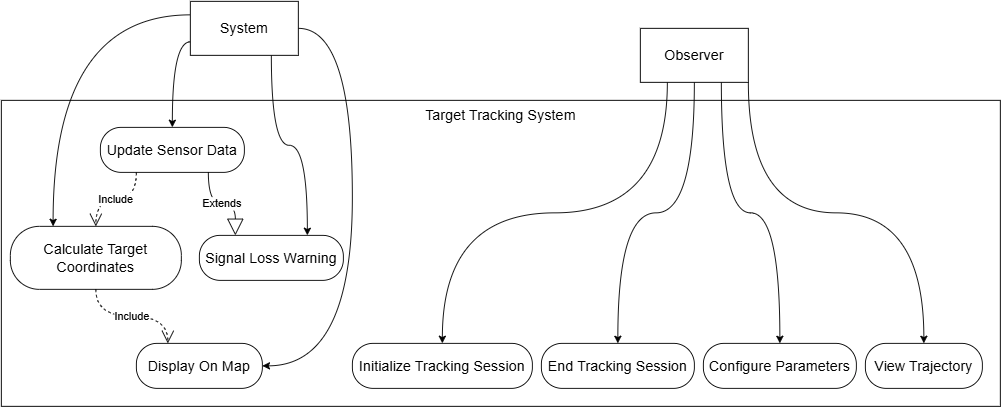
\includegraphics[width=0.85\textwidth]{Images/use-case-diagram.png}
\caption{Sơ đồ use-case của hệ thống tracking mục tiêu di động}
\label{fig:usecase-w1}
\end{figure}

Hệ thống tự động thực hiện các tác vụ nền: cập nhật dữ liệu cảm biến theo chu kỳ 10 Hz, tính toán tọa độ mục tiêu, áp dụng bộ lọc ước lượng, truyền tải kết quả qua kênh truyền dữ liệu hai chiều, hiển thị vị trí và quỹ đạo trên bản đồ, và cảnh báo khi mất tín hiệu cảm biến.

\subsubsection{Tóm tắt}

\hspace{0.5cm} Hệ thống bám mục tiêu di động thời gian thực được thiết kế theo hướng hợp nhất cảm biến laser, IMU và GNSS trên kiến trúc bốn tầng: cảm biến, nhúng, máy chủ và giao diện. Bài toán được phát biểu đầy đủ ở dạng hai chiều cho người đi bộ và xe máy, dạng ba chiều cho drone, với ngưỡng sai số thiết kế dưới 5,0 m. Phần cơ sở lý thuyết gồm chuỗi chuyển đổi tọa độ địa lý sang hệ tọa độ địa phương ENU, mô hình hợp nhất cảm biến theo trọng số nghịch đảo phương sai, và hai bộ lọc bám quỹ đạo là Kalman và alpha-beta. Kết quả kiểm chứng trên kịch bản mô phỏng chuẩn (seed = 42, thời lượng 120 giây, tần suất 10 Hz, bán kính vùng hoạt động 400 m) ghi nhận sai số RMSE đo thô 0,48 m cho người đi bộ, 1,89 m cho xe máy và 1,94 m cho drone; sau lọc, bộ lọc alpha-beta đưa các giá trị tương ứng về 0,26 m, 1,02 m và 1,06 m, bộ lọc Kalman về 0,86 m, 1,80 m và 2,10 m. Cả hai phương pháp đều thỏa ngưỡng thiết kế, trong khi alpha-beta cho sai số thấp hơn trong các kịch bản mô phỏng đã chạy.
